\documentclass[a4paper]{article}
\usepackage[english]{babel}
\usepackage[utf8x]{inputenc}
\usepackage{amsmath}
\usepackage{graphicx}
%%%%%%%%%%%%%%%%%%%%%%%%%%%%%%%
\title{AMORO Lab: Kinematics and Dynamics of a Biglide}
\author{} % Your name here
\date{} % Date of this report

\begin{document}
\maketitle
\begin{figure}[h!]
\centering
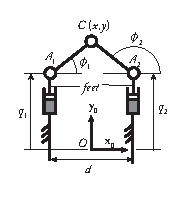
\includegraphics[width=0.6\textwidth]{PuRRRPu.eps}
\caption{Kinematic model of the Biglide}
\label{fig:biglide}
\end{figure}
\section{Model}
%
The kinematic architecture of the five-bar mechanism is shown in Fig.\ref{fig:biglide}. For the GAZEBO model, the geometric parameters are: 
\begin{itemize}
\item    $d=0.4$ m
\item    $l_{A1C}=0.3606$ m
\item    $l_{A2C}=0.3606$ m
\end{itemize}
The two prismatic joints are actuated. 

The base dynamic parameters are: 
\begin{itemize}
\item $m_p$ = 3 kg the mass of the end-effector
\item $m_f$ = 1 kg the mass of each foot
\end{itemize} 
All other dynamic parameters are neglected. 

%%%% From now, it is your work. 
\section{Geometric models}
%
\subsection{Direct geometric model}
%
\subsection{Passive joints geometric model}
%
\subsection{Inverse geometric model}
%%%%%%%%%%%%%%%%%%%%%%%
\section{First order kinematic models}
%
\subsection{Forward and inverse kinematic model}
%
\subsection{Passive joints kinematic model}
%%%%%%%%%%%%%%%%%%%%%%%
\section{Second order kinematic models}
%
\subsection{Forward and inverse kinematic model}
%
\subsection{Passive joints kinematic model}
%%%%%%%%%%%%%%%%%%%%%%%
\section{Dynamic model}
%
\end{document}
  



